\chapter{The ALICE experiment}
ALICE (\textit{A Large Ion Collider Experiment}) is one of the four major experiments at the \textit{Large Ion Collider}, at CERN, in Geneva. It was expressly designed to study heavy ion collisions, continuing the tradition of experiments such as STAR and PHENIX at RHIC, but also experiments held at SPS and AGS before. The aim of the experiment is the study of the QGP, using Pb-Pb collisions. However, ALICE has also a program with data from p-p and p-Pb collisions, needed to distinguish final state effects from initial states effects.\\
In this chapter a description of the experimental set up will be given, focusing on the \textit{Inner Tracking System}, after a brief introduction about the LHC.\\
\section{The Large Hadron Collider}
%
\begin{figure}
  \centering
  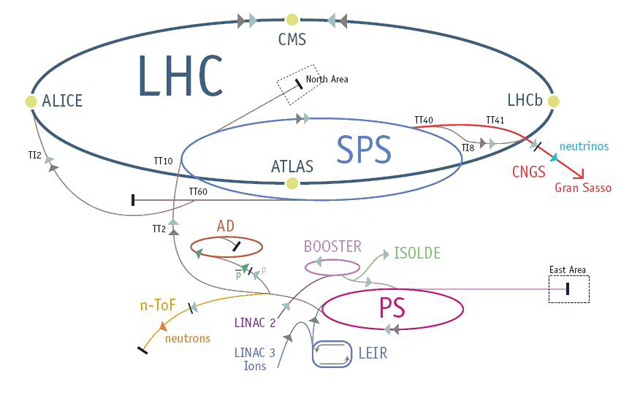
\includegraphics[scale=0.55]{figures/LHC.jpg}
  \caption{The accelerator complex at CERN.}
  \label{fig:LHC}
\end{figure}
%
The LHC is the world's largest and most powerful accelerator. It consists of a 27 km ring of superconducting magnets with a number of accelerating structures to boost the energy of the particles up to their collision energy and keep them stable, compensating the energy loss. The LHC is designed to deliver p-p collisions at $\sqrt{s}$ = 14 TeV, with a rate of 40 MHz, and Pb-Pb collisions at $\sqrt{s_{NN}}$ = 5.5 TeV, with a rate of 8 kHz. However, in the first run the LHC did not work at the highest energy, collecting mainly data for p-p collisions at $\sqrt{s}$ = 7 TeV and Pb-Pb collisions at $\sqrt{s_{NN}}$ = 2.76 TeV. In the second run, instead, the LHC is working at the design energies.\\
In Figure \ref{fig:LHC} a schematic view of the accelerator complex of CERN is shown. Protons and lead ions pass through different processes before reaching the LHC. Starting from protons, they are extracted from an hydrogen tank and injected in the linear accelerator LINAC2, where they reach an energy of 50 MeV. Then, they are accelerated to 1.4 GeV in the \textit{Proton Synchrotron Booster} (PSB) and injected in the \textit{Proton Synchrotron}, where they reach an energy of 25 GeV. Then, in the \textit{Super Proton Synchrotron} (SPS) they reach 450 GeV and are finally injected in the LHC. For lead ions the process is different, in particular in the initial steps. First of all, lead (Pb$^{208}$) ions are extracted from a purified sample of lead brought to high temperatures ($\sim$ 500 GeV) thanks to microwaves and the partially ionized by a stream of electrons, creating ions with different charges, among which only Pb$^{29+}$ are selected. After being accelerated in LINAC3 at 4.2 MeV per nucleon, more electrons are stripped by passing through a carbon foil. Only Pb$^{54+}$ are kept end then accelerated in the \textit{Low Energy Ion Ring} (LEIR) at 5.9 MeV. Then the ions are transferred to the PS, where they reach the energy of 5.9 GeV per nucleon end then pass through a copper foil, being fully stripped. The beam of Pb$^{82+}$ is then injected in the SPS (177 GeV per nucleon) and finally in the LHC, where they reach their final energy.
\section{Design considerations for ALICE}
The multiplicity of produced particles is a very important characteristic in the heavy ion collision experiments. For these kind of studies, indeed, it is important to track and identify all the particles coming from the interaction region, in order to measure the quantities described in the previous chapter. As already mentioned, the ALICE experiment was designed when RHIC data were not available yet, and the estimated multiplicity for heavy ion collision at the energy of the LHC was 2000 - 6000 particles for rapidity units. Consequently, the ALICE experiment has been designed in order to bear a multiplicity of 8000 particles for rapidity units. When the RHIC measurements became available, they showed that the multiplicity range at LHC should have been 1500 - 4000 particles for rapidity unit. Therefore, the designed was optimized for $\frac{dN}{dy}\sim$ 4000. Working at such a high values of multiplicity is possible thanks to the low interaction rate for heavy ions collisions, which allows to use slow detectors, such as the time projection chamber and the silicon drift detectors, which are very suitable for the particle identification. Another important parameter that have been taken into account in the design of the experiment is the efficiency, defined as the ratio between detected particles and generated particles. ALICE has full efficiency in $\varphi$, i.e. it covers $2\pi$ radians in the azimuthal angle.\\
ALICE, moreover, has been designed to work on a wide $p_T$ range. In facts, thanks to the mild magnetic field (0.5 T), it is possible to track particles down to very low values of transverse momentum (tens of MeV). This feature is ideal for the study of the soft probes, but the combination of the chosen magnetic field with the presence of the long lever arm, on which will be discussed later, allows precise momentum measurements even at high momentum ($p_T\lesssim$ 100 GeV/c).\\
Beside the reconstruction of the tracks of the particles, also the particle identification (PID) are extremely important, in order to reconstruct the particle spectra and get information about the QGP. At the ALICE experiment, the identification of particles with low transverse momentum (p < 4 GeV/c) is performed in the central barrel ($|\eta|$ < 0.9). For higher momenta, the particle identification can be done just in a restricted range of $\eta$ and $\varphi$ by specialized detectors and the measurement of the momentum has a reduced resolution, caused by the high bending radius of the particles.\\
